\chapter{Health, Load, and the Co-Founder}

The interview opens with a practical question about personal and mental health during the process of building a company. The answer unfolds in three steps. First, exercise is named as the obvious answer, and the speaker insists that the obvious answer is still true. Second, he points out why that answer is fragile: exercise is often the first thing a founder cuts when meetings and business pressure crowd the day. Third, he moves from private discipline to company design. A trusted co-founder changes how the work is carried.

\section{The Opening Question}

The question asks what steps the founder learned to take during the process of protecting personal and mental health. That phrasing matters. We are not beginning with an abstract wellness program. We are beginning with what remained useful inside the pressure of building a company.

The first object in the discussion is the founder under load. There is work to do, meetings to attend, responsibilities to divide, and a personal life that can still produce emergencies. The founder's problem is not only remembering to take care of himself. The deeper problem is that the business repeatedly gives him reasons to move the very practices that keep him durable.

\begin{definition}
A \emph{fungible commitment} is a commitment that a founder treats as easy to postpone when the day becomes crowded.
\end{definition}

The speaker's first example is exercise. He does not dismiss it as a cliché. He accepts it, and then immediately asks us to notice the pressure that makes it disappear.

\section{Exercise As The Obvious Answer}

The first answer is exercise. The speaker presents it as the answer people always return to, but he adds the important qualification: it really is true. Exercise is one of the ordinary supports of personal and mental health.

Then comes the turn. Exercise is also the thing people tend to cut first. A meeting appears. A business obligation feels urgent. The founder says that exercise can happen tomorrow. The practice is useful, but because it appears movable, it becomes the easiest thing to move.

\subsection{Question \& Answer}

\paragraph{Question.}
If exercise is the obvious answer, why does it disappear first?

\paragraph{Answer.}
Because it feels fungible. The cost of missing a meeting is immediate and visible. The cost of delaying exercise is slower, quieter, and easier to rationalize. So the founder trades away the thing that protects stamina in order to satisfy the thing that consumes stamina.

This is the local tension of the opening. The obvious answer is not wrong. It is just weak if it depends only on willpower. Once we see that, the next move is natural: we have to ask whether the company itself can be designed so that one founder is not carrying every load alone.

\section{From Habit To Structure}

The pivot is direct. Anyone looking for entrepreneurial work-life balance, the speaker says, should think seriously about partnering with somebody. This is not presented as a decorative form of encouragement. It is a structural answer to a structural problem.

A solo founder can become the company's single point of failure. If every task, meeting, emergency, and decision must pass through one person, then the founder's health and the company's capacity become too tightly coupled. A strong co-founder loosens that coupling.

\begin{figure}
\centering
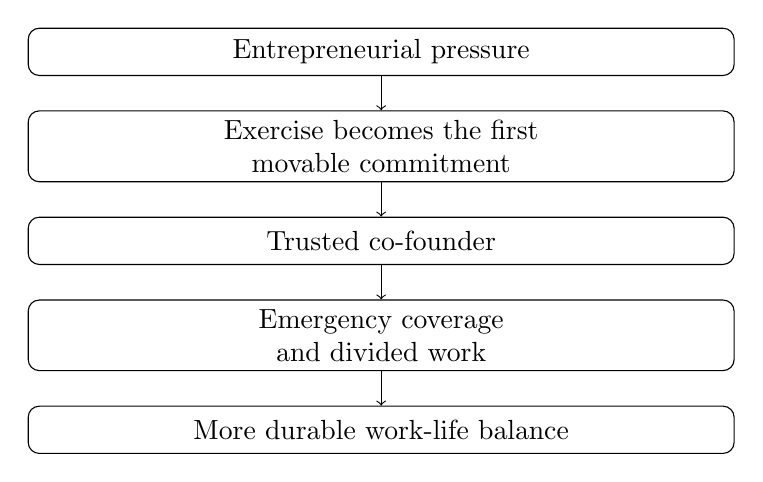
\begin{tikzpicture}
\node[draw, rounded corners, text width=0.72\linewidth, align=center, minimum height=0.60cm] (a) at (0,0) {Entrepreneurial pressure};
\node[draw, rounded corners, text width=0.72\linewidth, align=center, minimum height=0.60cm] (b) at (0,-1.20) {Exercise becomes the first\\movable commitment};
\node[draw, rounded corners, text width=0.72\linewidth, align=center, minimum height=0.60cm] (c) at (0,-2.40) {Trusted co-founder};
\node[draw, rounded corners, text width=0.72\linewidth, align=center, minimum height=0.60cm] (d) at (0,-3.60) {Emergency coverage\\and divided work};
\node[draw, rounded corners, text width=0.72\linewidth, align=center, minimum height=0.60cm] (e) at (0,-4.80) {More durable work-life balance};
\draw[->] (a) -- (b);
\draw[->] (b) -- (c);
\draw[->] (c) -- (d);
\draw[->] (d) -- (e);
\end{tikzpicture}
\end{figure}

This schematic is a compact reading of the interview's sequence. It is not a reproduced on-screen diagram. The important point is the direction of the argument: personal pressure exposes the limits of private discipline, and that opens the door to partnership as an operating structure.

\section{The Co-Founder As Operating Redundancy}

The speaker grounds the recommendation in founding experience. He says he could not have built the company without a strong co-partner. That is an anecdotal claim, but it is not vague. It is tied to a specific mechanism: two trusted partners can offload work for each other.

The transcript gives two concrete cases. First, there is the personal emergency. If one founder has to step away, the company does not have to stop. Second, there is the ordinary division of work. Even without a crisis, responsibility can be distributed.

\begin{proposition}
In this interview, the co-founder is not merely a source of encouragement. The co-founder is an operating redundancy: someone who can carry real work when the founder's own capacity is constrained.
\end{proposition}

\begin{proof}
The speaker moves from exercise to partnership only after explaining why founders cut the very habits that protect them. He then gives the concrete functions of the partner: covering personal emergencies and dividing work. Those functions reduce the company's dependence on one person's uninterrupted availability.
\end{proof}

That is the practical entrepreneurship lesson. A founder's health is not protected only by private discipline. It can also be protected by the architecture of responsibility inside the company.

\section{Trust, Enjoyment, and Different Skills}

After recommending partnership, the speaker immediately narrows the requirement. Finding somebody you trust is critical. The word carries operational weight. Offloading work only helps if delegation is safe. A partner who cannot be trusted does not reduce the burden; he becomes another burden.

The second criterion is enjoyment. This is not sentimentality. Building a company requires repeated coordination under stress. If the relationship itself is costly at every turn, the partnership can consume the same energy it was meant to preserve.

The third criterion is difference of skill. The transcript phrases this as complementary and even non-complementary skills. The safest reading is that each founder should bring something the other does not have. The point is not duplication. The point is expanded capacity.

\begin{remark}
The claim should stay modest. The speaker does not say that a co-founder guarantees balance, nor that every founder must choose the same kind of partner. He says that, in his own company-building experience, a strong co-partner made the work carryable.
\end{remark}

\section{A Compact Mechanism}

The interview gives us a mechanism rather than a formula. We can state it as a sequence of claims, each one close to the transcript:

\begin{enumerate}
\item Personal and mental health require practices that protect stamina.
\item Exercise is one of the obvious practices, and the speaker treats it as genuinely important.
\item Under business pressure, exercise is often treated as the first movable commitment.
\item The fragility of that habit reveals the limits of relying only on individual discipline.
\item A trusted co-founder changes the structure of the work.
\item Shared coverage makes personal emergencies less destructive.
\item Divided work makes the ordinary operating load less concentrated.
\item Trust, enjoyment, and different skills determine whether the partnership actually expands capacity.
\end{enumerate}

The distinction is between an individual remedy and a structural remedy. Exercise belongs to the individual remedy. Co-founder design belongs to the structural remedy. The speaker does not replace one with the other. He lets the weakness of the first reveal why the second matters.

\section{Summary}

The answer begins with exercise because the obvious answer is still true. It then shows why the obvious answer is hard to keep: founders often cut exercise first because it feels fungible beside meetings and urgent work. The deeper entrepreneurial lesson is structural. A trusted co-founder can absorb emergencies, divide work, and bring skills the founder lacks. Work-life balance, in this telling, is not only a private habit. It is also a design choice about how the company carries load.